\section{Architecture}
\subsection{Le système de fichiers}
\begin{frame}
\frametitle{Image de base}

\begin{itemize}
\item Busybox
\item Un serveur DHCP
\item Un deamon telnet
\item Un accès au port USB en mode série 
\end{itemize}

\end{frame}

\begin{frame}
\frametitle{Image de final}

\begin{itemize}
\item Un accès au port USB par connexion Ethernet
\item Le support du protocole SSH
\item La librairie DirectFB
\end{itemize}

\end{frame}

\subsection{Driver, ioctl et DirectFB}

\begin{frame}
\frametitle{Driver et ioctl}

Les fonctions ioctl du driver permettent :
\begin{itemize}
\item Mettre à jour l'affichage de l'écran
\item Récupérer des informations du driver (température, waveform ...)
\item Modifier des paramètres du driver (température, waveform ...)
\end{itemize}

\end{frame}

\begin{frame}
\frametitle{DirectFB}

\begin{itemize}
\item Fonction ioctl
\item Ensemble d'API graphiques
\item Interaction direct avec le framebuffer 
\item Aucune modification du kernel
\item Aucune dépendance (sauf libc mais déjà présent)
\end{itemize}

\end{frame}

\begin{frame}
\frametitle{Schéma fonctionnement DirectFB}

\begin{center}
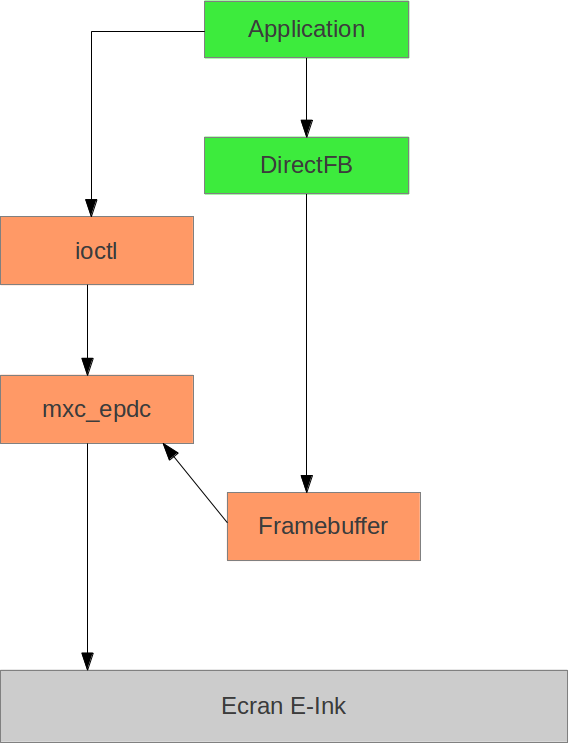
\includegraphics[scale=0.3]{schema_direct_fb.png}
\end{center}

\end{frame}

